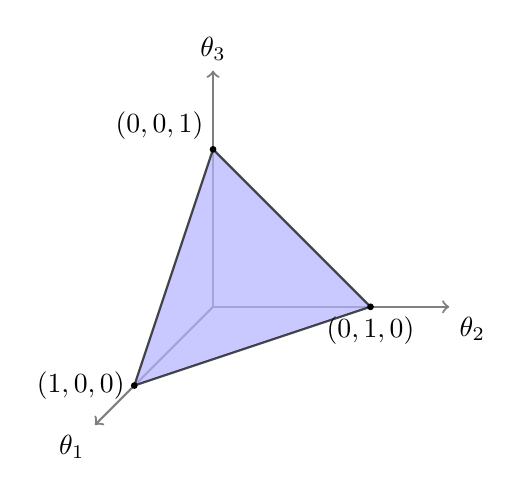
\begin{tikzpicture}[
    x={(-0.5cm,-0.5cm)}, 
    y={(1cm,0cm)}, 
    z={(0cm,1cm)}, 
    scale=2
]

    % Draw the axes
    \draw[->, thick, gray] (0,0,0) -- (1.5,0,0) node[anchor=north east, text=black] {$\theta_1$};
    \draw[->, thick, gray] (0,0,0) -- (0,1.5,0) node[anchor=north west, text=black] {$\theta_2$};
    \draw[->, thick, gray] (0,0,0) -- (0,0,1.5) node[anchor=south, text=black] {$\theta_3$};

    % Define the vertices of the simplex
    \coordinate (X) at (1,0,0);
    \coordinate (Y) at (0,1,0);
    \coordinate (Z) at (0,0,1);

    % Draw dashed lines from the origin to the vertices
    \draw[dashed, gray] (0,0,0) -- (X);
    \draw[dashed, gray] (0,0,0) -- (Y);
    \draw[dashed, gray] (0,0,0) -- (Z);

    % Draw the simplex plane (triangle)
    \draw[fill=blue!30, opacity=0.7, thick, join=round] (X) -- (Y) -- (Z) -- cycle;

    % Label the vertices
    \filldraw (X) circle (0.5pt) node[left] {$(1,0,0)$};
    \filldraw (Y) circle (0.5pt) node[below] {$(0,1,0)$};
    \filldraw (Z) circle (0.5pt) node[above left] {$(0,0,1)$};

\end{tikzpicture}